\section{Reachi Experiments}
\todo[inline]{introduce the data. WIP}
To verify that our model for computing path loss gives proper results, we have received data from conducted
experiments from the Reachi project. In total we have received data from four experiments. Three experiments
was conducted with 33 devices, while the fourth with 330.
% OMG SO BAAAAAD

\todo[inline]{talk about the problems with the data. WIP}
When we detected odd behaviour, we started to investigate the logs. Specifically the logs from experiments
conducted in Marikina and Rude skov. The reason for these two, is that the Rude skov log was not conducted in
the middle of a city while the Marikina was, as such the Marikina log should contain more varying signal
strength measurements because there is more dense obstructions that can influence the signal. We used the
distance dependent fading function from \cite{paper:linkmodel}, that computes path loss based on the distance of a
link, where we compared the measurements with transmission power - path loss computed from the distance fading
function.

On plot \ref{plot:reachi-experiments:average-distance} the measurements and distance fading function RSSI
values can be seen. The measurements have been divided into distance buckets, where the average for each
bucket has been computed and plotted.

\begin{figure}[H]
    \centering
    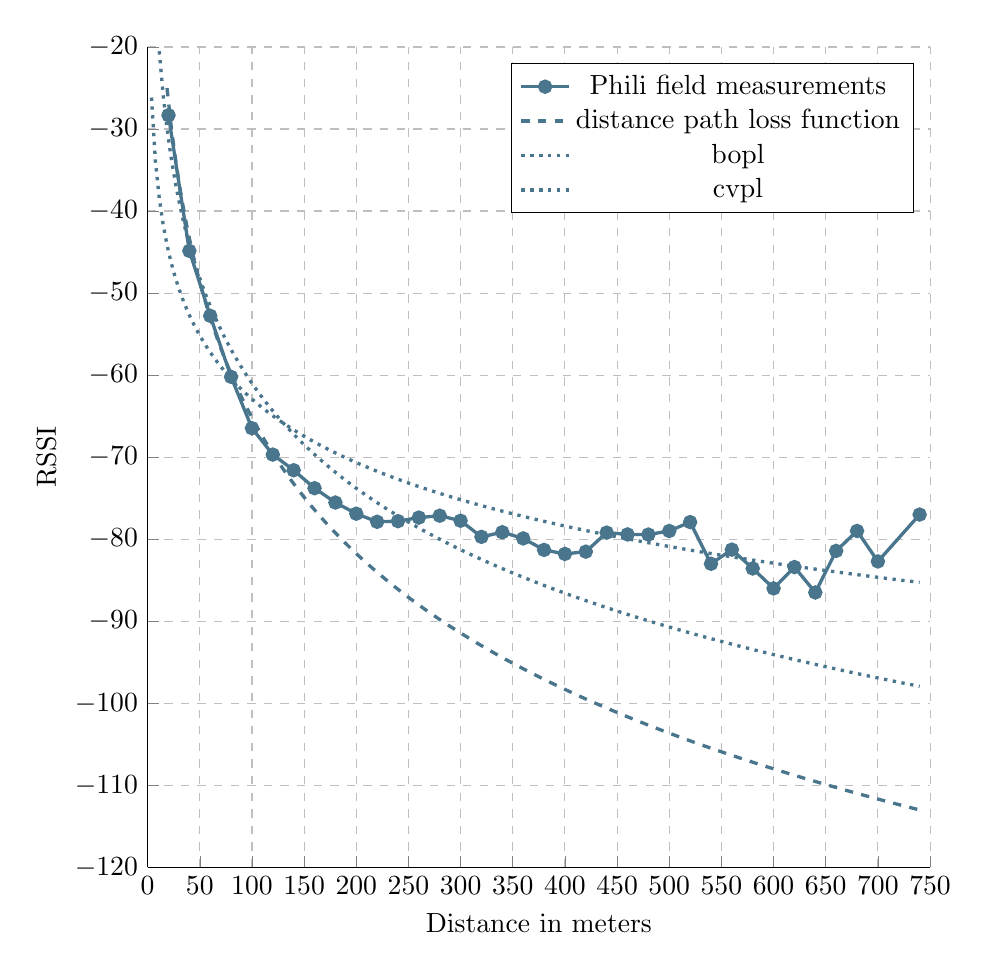
\begin{tikzpicture}%\label{plot:reachi-experiments:average-distance}
        \begin{axis}[
                height=12cm, width=0.95\textwidth,
                ylabel={RSSI},
                xlabel={Distance in meters},
                axis lines*=left,
                xmin=0, xmax=750,
                enlargelimits=false,
                ymin=-120, ymax=-20,
                xtick={0, 50, 100, 150, 200, 250, 300, 350, 400, 450, 500, 550, 600, 650, 700, 750},
                ymajorgrids=true,
                xmajorgrids=true,
                grid style=dashed,
                restrict y to domain=-120:-20,
                restrict x to domain=0:750,
                samples=200
            ]

            \addplot[very thick, solid, cyan!50!black, mark=*] coordinates {(20, -28.32345013477089) (40, -44.85830258302583) (60, -52.77323717948718) (80, -60.21201657458563) (100, -66.47435897435898) (120, -69.68905472636816) (140, -71.5976496922216) (160, -73.7866473149492) (180, -75.53428571428572) (200, -76.89289392378991) (220, -77.88135593220339) (240, -77.8035019455253) (260, -77.36784140969164) (280, -77.14030612244898) (300, -77.75299760191847) (320, -79.71686746987952) (340, -79.15481171548117) (360, -79.90728476821192) (380, -81.30909090909091) (400, -81.79746835443038) (420, -81.52272727272727) (440, -79.2) (460, -79.42105263157895) (480, -79.4375) (500, -79.0) (520, -77.91666666666667) (540, -83.0) (560, -81.27272727272727) (580, -83.57142857142857) (600, -86.0) (620, -83.4) (640, -86.5) (660, -81.42857142857143) (680, -79.0) (700, -82.71428571428571) (740, -77.0)};
            \addlegendentry{Phili field measurements};

        
            \addplot[domain=0:740, very thick, dashed, cyan!50!black] {26 - (55 * log10(x) -18.8)};
            \addlegendentry{distance path loss function};

            \addplot[domain=0:740, very thick, dotted, cyan!50!black] {26 - (42.5 * log10(x) + 2)};
            \addlegendentry{\gls{bopl}};

            \addplot[domain=0:740, very thick, dotted, cyan!50!black] {26 - (48.5 * (ln(x) / ln(77)) + 37.5)};
            \addlegendentry{\gls{cvpl}};
        \end{axis}
    \end{tikzpicture}
   \caption{Average RSSI pr. distance}%\label{plot:reachi-experiments:average-distance}
\end{figure}



\begin{figure}[H]
    \centering
    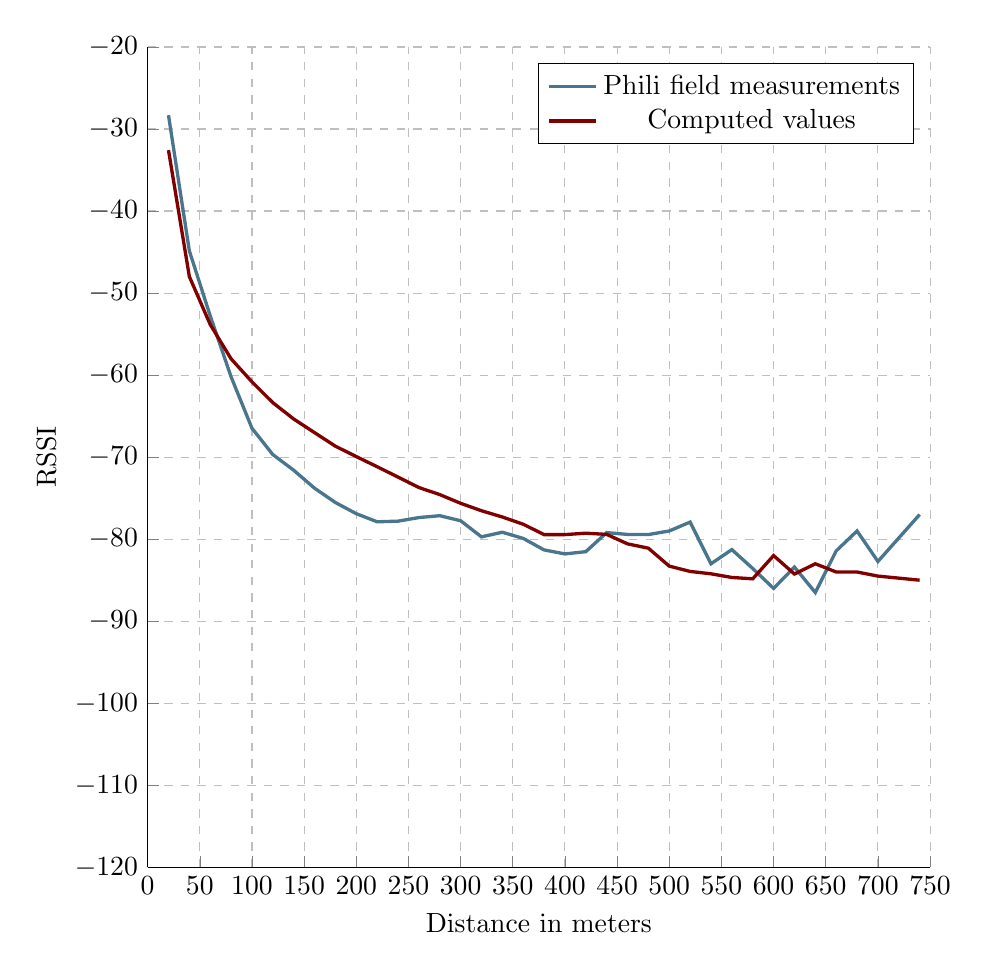
\begin{tikzpicture}%\label{plot:reachi-experiments:average-distance}
        \begin{axis}[
                height=12cm, width=0.95\textwidth,
                ylabel={RSSI},
                xlabel={Distance in meters},
                axis lines*=left,
                xmin=0, xmax=750,
                enlargelimits=false,
                ymin=-120, ymax=-20,
                xtick={0, 50, 100, 150, 200, 250, 300, 350, 400, 450, 500, 550, 600, 650, 700, 750},
                ymajorgrids=true,
                xmajorgrids=true,
                grid style=dashed,
                restrict y to domain=-120:-20,
                restrict x to domain=0:750,
                samples=200
            ]

            \addplot[very thick, solid, cyan!50!black] coordinates {(20, -28.32345013477089) (40, -44.85830258302583) (60, -52.77323717948718) (80, -60.21201657458563) (100, -66.47435897435898) (120, -69.68905472636816) (140, -71.5976496922216) (160, -73.7866473149492) (180, -75.53428571428572) (200, -76.89289392378991) (220, -77.88135593220339) (240, -77.8035019455253) (260, -77.36784140969164) (280, -77.14030612244898) (300, -77.75299760191847) (320, -79.71686746987952) (340, -79.15481171548117) (360, -79.90728476821192) (380, -81.30909090909091) (400, -81.79746835443038) (420, -81.52272727272727) (440, -79.2) (460, -79.42105263157895) (480, -79.4375) (500, -79.0) (520, -77.91666666666667) (540, -83.0) (560, -81.27272727272727) (580, -83.57142857142857) (600, -86.0) (620, -83.4) (640, -86.5) (660, -81.42857142857143) (680, -79.0) (700, -82.71428571428571) (740, -77.0)};
            \addlegendentry{Phili field measurements};

            \addplot[very thick, solid, red!50!black] coordinates {(20, -32.57699443413729) (40, -47.990196078431374) (60, -53.83796296296296) (80, -58.01576872536137) (100, -60.821969696969695) (120, -63.358533791523485) (140, -65.34886025768087) (160, -67.01231527093596) (180, -68.66666666666667) (200, -69.9340490797546) (220, -71.1676891615542) (240, -72.43023255813954) (260, -73.70394736842105) (280, -74.56488549618321) (300, -75.62758620689655) (320, -76.53333333333333) (340, -77.29651162790698) (360, -78.18018018018019) (380, -79.44186046511628) (400, -79.44262295081967) (420, -79.27272727272727) (440, -79.41666666666667) (460, -80.57142857142857) (480, -81.1) (500, -83.28571428571429) (520, -83.93333333333334) (540, -84.22222222222223) (560, -84.66666666666667) (580, -84.83333333333333) (600, -82.0) (620, -84.25) (640, -83.0) (660, -84.0) (680, -84.0) (700, -84.5) (740, -85.0)};
            \addlegendentry{Computed values};
        \end{axis}
    \end{tikzpicture}
   \caption{Field measurements vs computed values}%\label{plot:reachi-experiments:dsa}
\end{figure}



\begin{figure}[H]
    \centering
    \begin{tikzpicture}%\label{plot:reachi-experiments:average-distance}
        \begin{axis}[
                height=12cm, width=0.95\textwidth,
                ylabel={RSSI},
                xlabel={Distance in meters},
                axis lines*=left,
                xmin=0, xmax=380,
                enlargelimits=false,
                ymin=-90, ymax=-30,
                % xtick={0, 50, 100, 150, 200, 250, 300, 350, 400, 450, 500, 550, 600, 650, 700, 750},
                ymajorgrids=true,
                xmajorgrids=true,
                grid style=dashed,
                restrict y to domain=-90:-30,
                restrict x to domain=0:380,
                samples=700
            ]

            \addplot[very thick, solid, cyan!50!black] coordinates {(20, -32.56521739130435) (40, -50.607142857142854) (60, -52.15384615384615) (80, -64.85714285714286) (100, -49.5) (120, -65.76623376623377) (140, -69.38888888888889) (160, -72.05714285714286) (180, -69.3125) (200, -78.83333333333333) (220, -76.84) (240, -75.75) (260, -80.91666666666667) (280, -72.88888888888889) (300, -78.95238095238095) (320, -76.44444444444444) (340, -82.75) (380, -87.0)};
            \addlegendentry{Phili field measurements}


            \addplot[domain=0:380, very thick, solid, red!50!black] {26 - bopl(x)};
            \addlegendentry{\gls{bopl}};

       
        \end{axis}
    \end{tikzpicture}
   \caption{Field measurements with building percentage above 80\%}%\label{plot:reachi-experiments:dsa}
\end{figure}


\begin{figure}[H]
    \centering
    \begin{tikzpicture}%\label{plot:reachi-experiments:average-distance}
        \begin{axis}[
                height=12cm, width=0.95\textwidth,
                ylabel={RSSI},
                xlabel={Distance in meters},
                axis lines*=left,
                xmin=0, xmax=750,
                enlargelimits=false,
                ymin=-90, ymax=-30,
                xtick={0, 50, 100, 150, 200, 250, 300, 350, 400, 450, 500, 550, 600, 650, 700, 750},
                ymajorgrids=true,
                xmajorgrids=true,
                grid style=dashed,
                restrict y to domain=-90:-30,
                restrict x to domain=0:750,
                samples=700
            ]

            \addplot[very thick, solid, cyan!50!black] coordinates {(20, -36.01344537815126) (40, -48.361111111111114) (60, -54.93279022403259) (80, -62.40816326530612) (100, -68.14871794871794) (120, -60.85954712362301) (140, -71.69568452380952) (160, -74.36896551724138) (180, -73.93817204301075) (200, -75.09929078014184) (220, -73.38403041825094) (240, -75.43994413407822) (260, -77.69102990033223) (280, -77.31512605042016) (300, -75.7751937984496) (320, -78.60714285714286) (340, -78.38524590163935) (360, -78.52459016393442) (380, -77.34285714285714) (400, -80.96153846153847) (420, -81.03571428571429) (440, -80.41379310344827) (460, -74.18181818181819) (480, -79.9090909090909) (500, -79.75) (520, -77.56521739130434) (540, -81.23076923076923) (560, -78.9) (580, -85.0) (620, -82.5) (640, -82.33333333333333) (660, -82.4) (680, -77.5) (700, -85.4) (740, -77.0)};
            \addlegendentry{Phili field measurements}


            \addplot[domain=0:740, very thick, solid, red!50!black] {26 - cvpl(x)};
            \addlegendentry{\gls{cvpl}};

       
        \end{axis}
    \end{tikzpicture}
   \caption{Field measurements with building percentage below 5\%}%\label{plot:reachi-experiments:dsa}
\end{figure}



\begin{figure}[H]
    \centering
    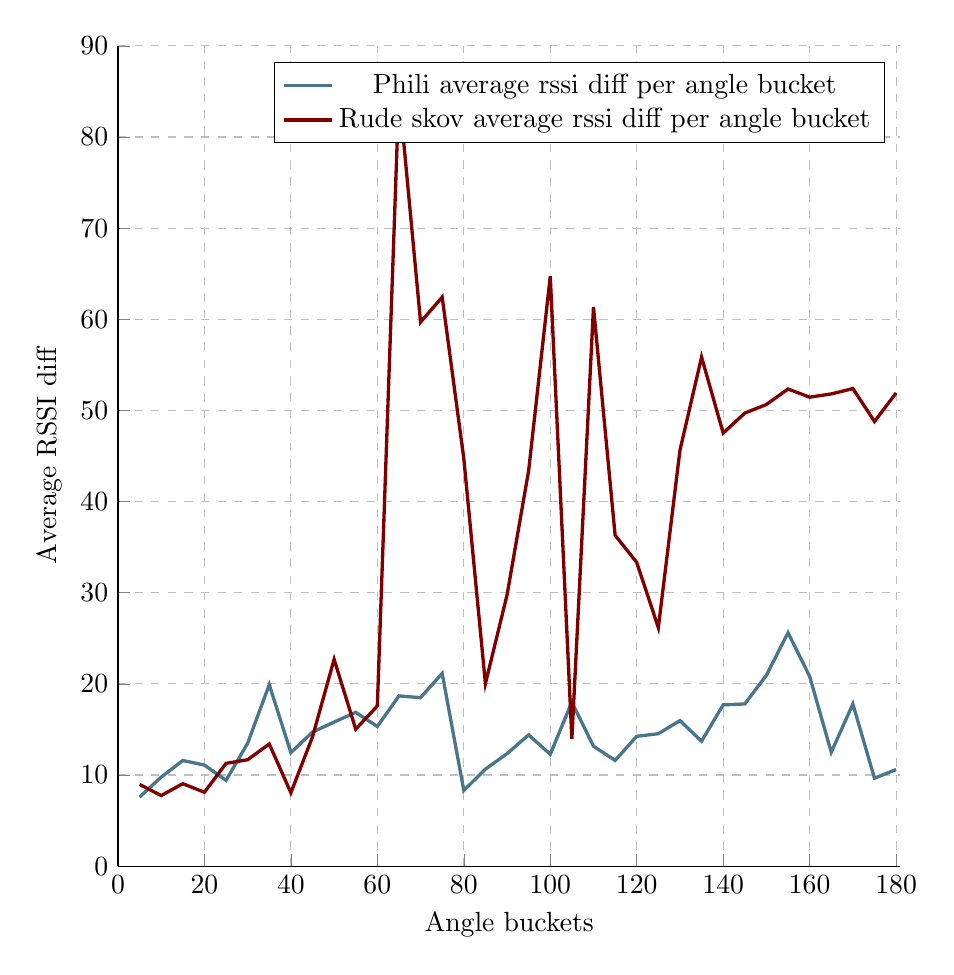
\begin{tikzpicture}%\label{plot:reachi-experiments:average-distance}
        \begin{axis}[
                height=12cm, width=0.95\textwidth,
                ylabel={Average RSSI diff},
                xlabel={Angle buckets},
                axis lines*=left,
                xmin=0, xmax=181,
                enlargelimits=false,
                ymin=0, ymax=90,
                % xtick={0, 50, 100, 150, 200, 250, 300, 350, 400, 450, 500, 550, 600, 650, 700, 750},
                ymajorgrids=true,
                xmajorgrids=true,
                grid style=dashed
                % restrict y to domain=0:25,
                % restrict x to domain=0:180
            ]

            \addplot[very thick, solid, cyan!50!black] coordinates {(5, 7.581215097994852) (10, 9.763581254686114) (15, 11.59234807189617) (20, 11.084399582147876) (25, 9.411670936293284) (30, 13.486232393853125) (35, 19.91110051641767) (40, 12.453590557884946) (45, 14.70313120243339) (50, 15.804939314638208) (55, 16.87697870999425) (60, 15.320902904198922) (65, 18.673392004683087) (70, 18.48508963612783) (75, 21.147550183881993) (80, 8.302184073487094) (85, 10.641508684206432) (90, 12.343183048128944) (95, 14.396643466792797) (100, 12.27504884861337) (105, 17.994872329043496) (110, 13.156645245862158) (115, 11.595967499573286) (120, 14.245146945189493) (125, 14.528392002600814) (130, 15.96981736460891) (135, 13.70427190114752) (140, 17.692009757218077) (145, 17.79486440192431) (150, 20.947579654378668) (155, 25.611175147469265) (160, 20.819124899373364) (165, 12.495568407794714) (170, 17.784042978338544) (175, 9.646875797269503) (180, 10.597197732034614)};
            \addlegendentry{Phili average rssi diff per angle bucket};


            \addplot[very thick, solid, red!50!black] coordinates {(5, 8.968175725354994) (10, 7.741408675352775) (15, 9.042742837449076) (20, 8.108954051047618) (25, 11.273321343260399) (30, 11.67692967914715) (35, 13.401460743255232) (40, 8.053793318539391) (45, 14.17474549040368) (50, 22.68855220716477) (55, 15.026896145186285) (60, 17.5755161176863) (65, 85.01233086400362) (70, 59.69038212814202) (75, 62.41948703096457) (80, 44.72712810089782) (85, 20.029080610052482) (90, (29.737954905927445) (95, 43.39235466255519) (100, 64.720015835849) (105, 13.965589072181558) (110, 61.334883149884675) (115, 36.30455538419785) (120, 33.32223486902817) (125, 26.172354285886417) (130, 45.62355888699502) (135, 55.8474401182669) (140, 47.511612928722954) (145, 49.70429537245245) (150, 50.649080550831435) (155, 52.34402139529124) (160, 51.45218633523966) (165, 51.805898996936115) (170, 52.39131328924595) (175, 48.78102582759046) (180, 51.91529108595685)};
            \addlegendentry{Rude skov average rssi diff per angle bucket};
        \end{axis}
    \end{tikzpicture}
   \caption{}%\label{plot:reachi-experiments:dsa}
\end{figure}



\todo[inline]{show some plots, proving the problems}
\todo[inline]{talk about the visualiser + youtube link that shows the problems}
\todo[inline]{shortly mention CVPL and BOPL model that will be introduced in detail later}